\lchapter[intro]{Introduction}

\section{Complex engineering systems}

\p{Complex systems}
A complex system is a system composed of many heterogeneous connected entities that as a whole present a behavior which cannot be predicted by studying the single entities by themselves. Normally, a complex system, is composed by a large number of entities (in the order of at least \numprint{1e3}). According to \citeauthor{systcomplex} \cite{systcomplex}, complex systems can be categorized into \emph{disorganized complexity} and \emph{organized complexity}. The first category is used to refer to very large but easy to understand systems, for which answers to particular questions can be given with high precision. The second category is used to refer to systems presenting an emerging behavior which cannot be analyzed with the same statistical tools used to answer questions about disorganized systems.

\p{Complex engineering systems}
\emph{Engineering systems} are a class of systems characterized by a high degree of technical complexity, social intricacy, and elaborate processes, aimed at fulfilling important functions in society \cite{complex}. When an engineering system is complex enough to meet the definition of a complex system, that is, for example, when many engineers contribute to a project with many components, we can classify it as a \emph{complex engineering system}.

\p{Graph modeling}
According to \citeauthor{decomp} \cite{decomp}, \citeauthor{complex} \cite{complex}, and \citeauthor{change-prop} \cite{change-prop}, such complex systems can be understood as a set of tightly coupled layered subsystems. This decomposition can then be represented as a multi-layer graph, where vertices represent entities (components, engineers, resources, processes,\ldots) and edges represent interactions between these entities. Entities belonging to the same category are placed on the same layer. \Vref{fig:citynet} contains an example of such a modeling. \Ref{fig:citynet-energy} shows the energy-related interdependencies for a city. \Ref{fig:citynet-layers} shows a sample energy configuration with the different layers placed over the city's map \cite{citynet}.

\begin{figure}[!h]
\begin{adjustwidth}{0cm}{0cm}
  	\subfloat[Energy-related interdependencies]{
		\label{fig:citynet-energy}
		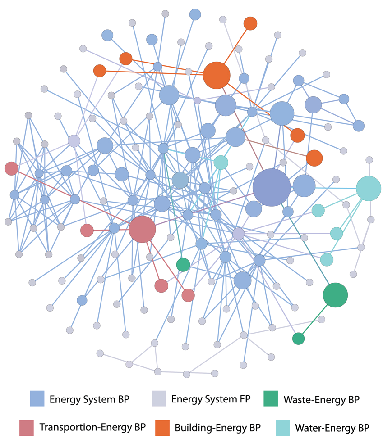
\includegraphics[width=.315\linewidth]{images/citynet-energy}
	}
	\hspace{1.7cm}
	\subfloat[Sample energy configuration]{
		\label{fig:citynet-layers}
		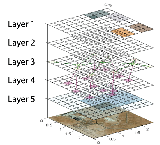
\includegraphics[width=.38\linewidth]{images/citynet-layers}
	}
	\caption[Example energy-related interdependencies for a city and a 3-D rendering superposed to an actual map.]{Example energy-related interdependencies for a city and a 3-D rendering superposed to an actual map. Source: \cite{citynet}.}
	\label{fig:citynet}
\end{adjustwidth}
\end{figure}

\section{Data collection}
\label{sec:intro/collection}

\p{Tangible systems}
The process of modeling, visualizing, and analyzing any type of system, whether complex or not, presupposes the availability of the data set describing the system itself, and optionally, the processes contributing to its evolution. When modeling tangible systems such as aircrafts or cities, the data collection process becomes rapidly very onerous and imprecise.

\p{Intangible systems}
On the other hand, when the system under exam is intangible and essentially composed by information, it is possible to process it automatically and obtain more precise data in much less time. The typical example of such a system is a software code \cite{mc1,mc2,mc3}. Additionally, different tools are already used in the industry to collect additional data about the processes contributing to its development, as for example bug trackers, wikis, or email communication.

\p{Open-source software}
Another particularity of the software world is the \gls{oss} movement. As this software is developed by many people around the world, not only the source code is freely available for inspection, but so is the information stored by the tools that the developers use to collaborate with the community.

\p{Using software as a proxy system}
By choosing to focus our analysis on complex software projects, we greatly facilitate the data collection and processing tasks, and can concentrate our efforts on the core problem. We assume that when data about a different (tangible) system becomes available, the very same process can be used to analyze or visualize it as well.

\section{Graph visualization}
\label{sec:intro/visu}

\p{Graph visualization}
A widespread problematic when working with graphs is how to automatically lay them out to be visualized for consumption by human beings, i.e., deciding which vertex has which position, and how the lines representing edges are drawn. Different types of graphs may need different drawing conventions, and different users may like to emphasize different aspects of the data \cite{graphdraw,graphvisu}. Many approaches and many solutions exist to this problem.

\p{Complex systems visualization}
By modeling complex systems using multi-domain networks, we can exploit the extensive academic background in graph drawing to visualize complex systems \cite{alg1,alg2,alg3,alg4}. Different graph visualization applications and libraries exists, but none of them are specifically oriented towards the visualization of multi-domain networks. Various graph visualization applications making use of these layout algorithms have already been documented, but because they are using layout algorithms as their building blocks, built-in support for multi-domain data is absent from all of them.

\section{Project goals}
\label{sec:intro/goals}
\p{Goal of the project}
The goal of this project is to provide an approach, software architecture and software code to visualize any complex system modeled using a multi-domain network. The final intended result is an easy to use, portable, and extensible application specifically oriented towards multi-domain datasets.

\p{Analysis of open-source software}
As stated in the preceding sections, the collection of data about a given system can be a cumbersome task. To facilitate the aggregation of different data sets to be able to test and evaluate the application, we decided to focus our analysis on open-source software projects. As consequence of this decision, the application to be developed shall support an easy way to gather data about a given software project in an automated and extensible fashion.

\p{Layout algorithms}
Additionally, as part of the visualization application, we will have to research and implement different layout algorithms (or techniques based on them) to place the nodes of a multi-domain network on a surface or in space in an appropriate way and by considering the intrinsic nature of the modeled system.

\p{More information}
Additional information about the project goal are available in the complete project statement in \vref{sec:statement}.

\section{Execution context}

This work is carried out at the \gls{mit} during the spring semester 2013 and is valid as Master Thesis for the accomplishment of the regular master course for the \emph{Master of Science in Engineering}, major in \emph{Information and Communication Technologies}, at the \gls{hesso}//Master.

This project is heavily based on the \emph{Graph Visualization Optimization} semester project carried out during the previous term at the \gls{eiafr}.

Prof. Pierre Kuonen of \gls{eiafr}, Switzerland, is the project supervisor. Prof. Olivier L. de Weck, Associate Professor of Aeronautics and Astronautics and Engineering Systems at \gls{mit}, USA, is the assigned expert for the project.

\section{Structure of this document}

This document is structured in five chapters as follows:

\begin{itemize}
  \item \Ref*{sec:intro} is the global introduction to the report.
  \item \Vref*{sec:case} presents the initial case study and contains an overview of the state of the art and the adopted overall system architecture.
  \item \Vref*{sec:acquisition} focuses on the data acquisition framework developed as part of the project.
  \item \Vref*{sec:visu} is the main chapter of the report and focuses on the data visualization web application.
  \item \Vref*{sec:conclusions} contains the conclusions to the report.
\end{itemize}

Additionally, 3 appendices are available to provide additional content. They are structured as follows:

\begin{itemize}
  \item \Vref*{sec:graphml} provides a listing of the limitations of the GraphML specification.
  \item \Ref*{sec:statement} includes the original project statement.
  \item \Ref*{sec:cdrom} lists the content available on the attached \gls{cd-rom}.
\end{itemize}
